\documentclass{article}\usepackage[]{graphicx}\usepackage[]{xcolor}
% maxwidth is the original width if it is less than linewidth
% otherwise use linewidth (to make sure the graphics do not exceed the margin)
\makeatletter
\def\maxwidth{ %
  \ifdim\Gin@nat@width>\linewidth
    \linewidth
  \else
    \Gin@nat@width
  \fi
}
\makeatother

\definecolor{fgcolor}{rgb}{0.345, 0.345, 0.345}
\newcommand{\hlnum}[1]{\textcolor[rgb]{0.686,0.059,0.569}{#1}}%
\newcommand{\hlstr}[1]{\textcolor[rgb]{0.192,0.494,0.8}{#1}}%
\newcommand{\hlcom}[1]{\textcolor[rgb]{0.678,0.584,0.686}{\textit{#1}}}%
\newcommand{\hlopt}[1]{\textcolor[rgb]{0,0,0}{#1}}%
\newcommand{\hlstd}[1]{\textcolor[rgb]{0.345,0.345,0.345}{#1}}%
\newcommand{\hlkwa}[1]{\textcolor[rgb]{0.161,0.373,0.58}{\textbf{#1}}}%
\newcommand{\hlkwb}[1]{\textcolor[rgb]{0.69,0.353,0.396}{#1}}%
\newcommand{\hlkwc}[1]{\textcolor[rgb]{0.333,0.667,0.333}{#1}}%
\newcommand{\hlkwd}[1]{\textcolor[rgb]{0.737,0.353,0.396}{\textbf{#1}}}%
\let\hlipl\hlkwb

\usepackage{framed}
\makeatletter
\newenvironment{kframe}{%
 \def\at@end@of@kframe{}%
 \ifinner\ifhmode%
  \def\at@end@of@kframe{\end{minipage}}%
  \begin{minipage}{\columnwidth}%
 \fi\fi%
 \def\FrameCommand##1{\hskip\@totalleftmargin \hskip-\fboxsep
 \colorbox{shadecolor}{##1}\hskip-\fboxsep
     % There is no \\@totalrightmargin, so:
     \hskip-\linewidth \hskip-\@totalleftmargin \hskip\columnwidth}%
 \MakeFramed {\advance\hsize-\width
   \@totalleftmargin\z@ \linewidth\hsize
   \@setminipage}}%
 {\par\unskip\endMakeFramed%
 \at@end@of@kframe}
\makeatother

\definecolor{shadecolor}{rgb}{.97, .97, .97}
\definecolor{messagecolor}{rgb}{0, 0, 0}
\definecolor{warningcolor}{rgb}{1, 0, 1}
\definecolor{errorcolor}{rgb}{1, 0, 0}
\newenvironment{knitrout}{}{} % an empty environment to be redefined in TeX

\usepackage{alltt}
\usepackage[utf8]{inputenc}
\usepackage{amsfonts}
\usepackage{tgpagella}
\usepackage{graphicx} % Required for inserting images
\usepackage{polski}
\renewcommand*{\figurename}{Rysunek}
\usepackage{nicefrac, xfrac}
\usepackage[margin=1in]{geometry}
\usepackage{hyperref}
\usepackage{xcolor}
\usepackage{amssymb}
\usepackage[bottom]{footmisc}
\usepackage{float}
\IfFileExists{upquote.sty}{\usepackage{upquote}}{}
\begin{document}



\section{Liczba naprawianych pojazdów w każdym miesiącu pracy warsztatu}

{\color{red}[jakiś wstęp do tego]}

\begin{knitrout}
\definecolor{shadecolor}{rgb}{0.969, 0.969, 0.969}\color{fgcolor}\begin{figure}[h]

{\centering 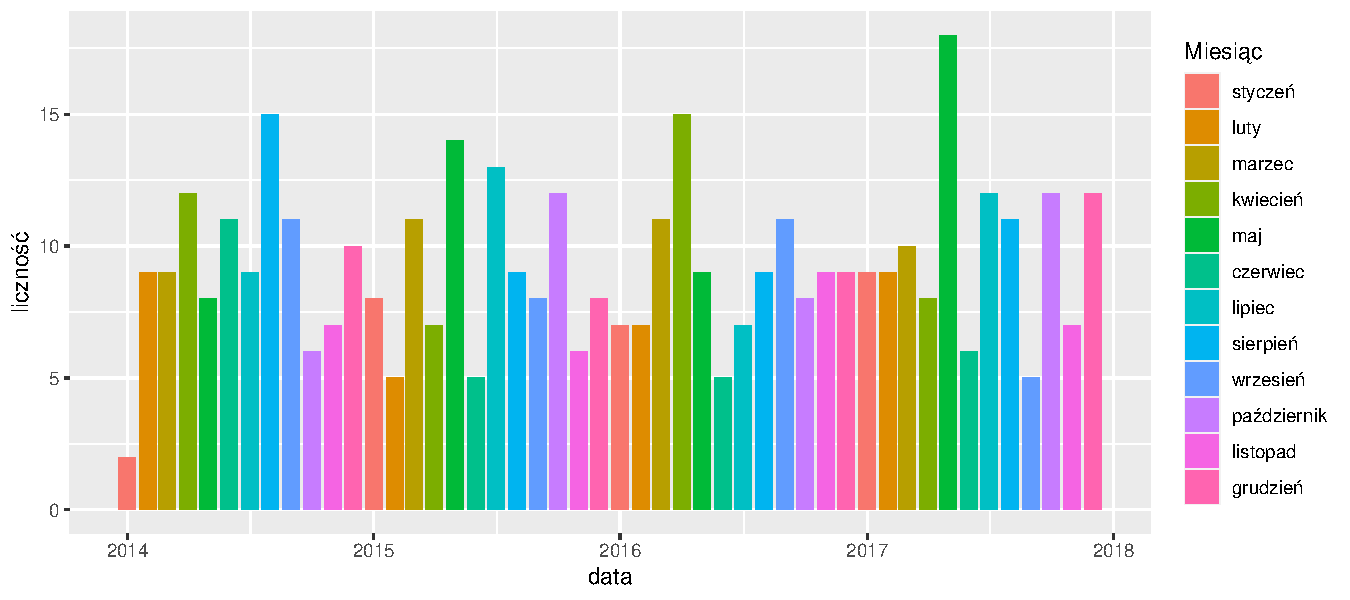
\includegraphics[width=\maxwidth]{figure/fig_naprawy_miesiecznie-1} 

}

\caption[Wykres liczba naprawianych pojazdów w każdym miesiącu pracy warsztatu]{Wykres liczba naprawianych pojazdów w każdym miesiącu pracy warsztatu}\label{fig:fig_naprawy_miesiecznie}
\end{figure}

\end{knitrout}

Wykres \ref{fig:fig_naprawy_miesiecznie} przedstawia liczbę naprawionych pojazdów w każdym miesiącu pracy warsztatu. Najwięcej pojazdów zostało naprawionych w miesiącach: 
maj 2017,
a było ich 18. Natomiast najmniej przeprowadzonych napraw było w miesiącach:
styczeń 2014,
było ich 2. Średnia liczba napraw miesięcznie wynosi 
9.188. 

\section{Profil klienta}

W następnej koljeności zostaną przeanalizawani klienci warsztatu. Zostaną sprawdzone liczności klientów ze względu na różne ich cechy. {\color{red}[Czy warto pisać, że może nam to pomóc stwierdzić, do jakich klientów moglibyśmy spróbować jeszcze dotrzeć.]}

\subsection{Płeć}

Pierwszą cechą jaka zostanie wzięta pod uwagę jest płeć klienta.

\begin{knitrout}
\definecolor{shadecolor}{rgb}{0.969, 0.969, 0.969}\color{fgcolor}\begin{figure}

{\centering 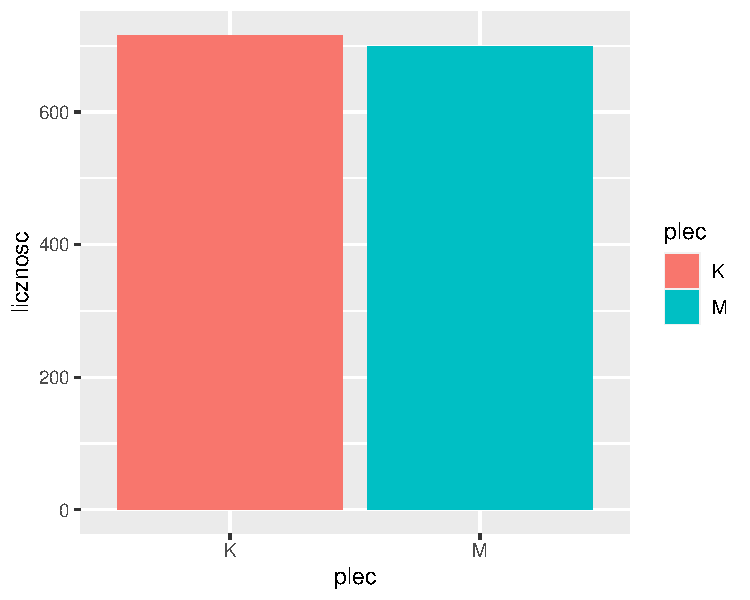
\includegraphics[width=\maxwidth]{figure/fig_plec-1} 

}

\caption[Wykres liczby klientów przy podziale ze względu na płeć]{Wykres liczby klientów przy podziale ze względu na płeć}\label{fig:fig_plec}
\end{figure}

\end{knitrout}

Na wykresie słupkowym \ref{fig:fig_plec} są zaprezentowane liczności klientów przy podziale ze względu na płeć. Więcej klientów warsztatu należy do grupy kobiet. Grupa kobiet jest około 1.102
razy większa od grupy mężczyzn, a zatem różnica jest nie duża.

\subsection{Wiek}

Zostanie również przeanalizowany rozkład wieku klientów warsztatu.





\begin{knitrout}
\definecolor{shadecolor}{rgb}{0.969, 0.969, 0.969}\color{fgcolor}\begin{figure}

{\centering 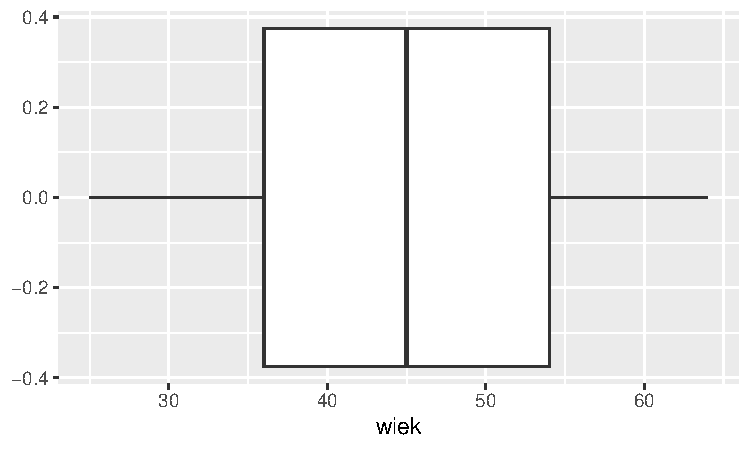
\includegraphics[width=\maxwidth]{figure/fig_wiek-1} 

}

\caption[Wykres pudełkowy wieku klientów]{Wykres pudełkowy wieku klientów}\label{fig:fig_wiek}
\end{figure}

\end{knitrout}

Rysunek \ref{fig:fig_wiek} przedstawia wykres pudełkowy wieku klientów warsztatu. Widać, że mediana wynosi [mediana], natomiast pierwszy kwartyl wynosi {\color{red}[Q1]}, trzeci kwartyl natomiast {\color{red}[Q3]}. {\color{red}[Mogłabym coś napisać, który jest bardziej oddalony od mediany]}. Najmłodszy klient warsztatu ma {\color{red}[najmniejszy wiek]}, natomiast najstarszy klient ma {\color{red}[najwyższy wiek]}.

\begin{table}[H]
\centering
\begin{tabular}{c|c} \hline
Miara & Wartość \\ \hline
Średnia & 45.17 \\ 
Odchylenie standardowe & 10.73 \\
Skośność & 0.02  \\ 
Kurtoza & 1.86 \\ \hline
\end{tabular}
\caption{Wybrane miary wieku klientów}
\label{tab_wiek}
\end{table}

Kilka miar, których nie da się odczytać z wykresu, zostało przedstawionych w tabli \ref{tab_wiek}. Można zatem odczytać, że średnio klieci mają 45.17, a odchylenie standardowe wieku wynoski 10.73. {\color{red}[Zdanie że średnia jest mniejsza/podobna/większa a zatem jakaś skośność, co potwierdza współczynnik skośności]}

\subsection{Miasto}
\begin{knitrout}
\definecolor{shadecolor}{rgb}{0.969, 0.969, 0.969}\color{fgcolor}\begin{kframe}
\begin{verbatim}
##         miasto liczność
## 1      Wrocław      708
## 2    Bydgoszcz       22
## 3         Łódź       20
## 4 Zielona Góra       16
## 5       Poznań       16
## 6        Opole       16
\end{verbatim}
\end{kframe}
\end{knitrout}

[opis tabelki]

\subsection{Karta lojalnościowa}
\begin{knitrout}
\definecolor{shadecolor}{rgb}{0.969, 0.969, 0.969}\color{fgcolor}\begin{figure}

{\centering 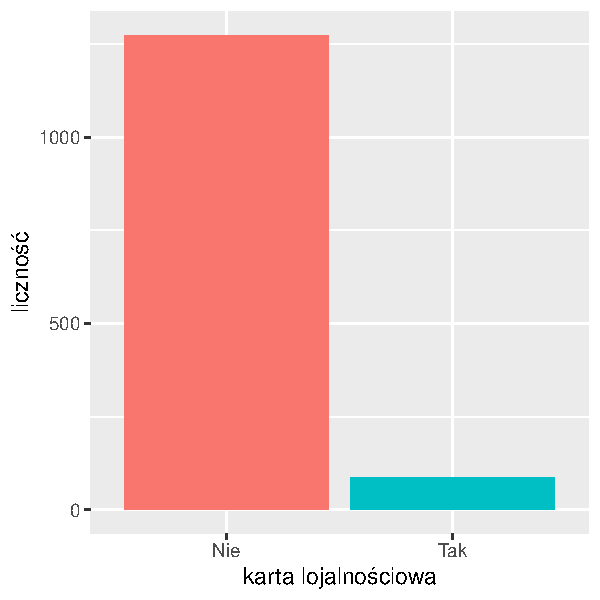
\includegraphics[width=\maxwidth]{figure/fig_karta-1} 

}

\caption[Wykres liczby klientów ze względu na posiadanie karty lojalnościowej]{Wykres liczby klientów ze względu na posiadanie karty lojalnościowej}\label{fig:fig_karta}
\end{figure}

\end{knitrout}

\section{Tabela najlepszych okazji}





\begin{knitrout}
\definecolor{shadecolor}{rgb}{0.969, 0.969, 0.969}\color{fgcolor}\begin{kframe}
\begin{verbatim}
##     id_samochodu         marka    model   zysk
## 636          742 Mercedes-Benz E 63 AMG 126558
## 497          592       Porsche Panamera  99182
## 175          221 Mercedes-Benz    E 300  98044
## 805          779        Jaguar      XKR  87200
## 881          969       Porsche Panamera  82355
## 716          817          Audi      RS3  76412
\end{verbatim}
\end{kframe}
\end{knitrout}

\section{Jak wybrane cechy pojazdów wpływają na zysk warsztatu? (zastanowić się nad tytułem !!!)}

\subsection{Rodzaj pojazdu}

{\color{red}[Skupimy się, czy to samochód czy motocykl]}

[tabelka z miarami ???]

\begin{knitrout}
\definecolor{shadecolor}{rgb}{0.969, 0.969, 0.969}\color{fgcolor}\begin{figure}

{\centering 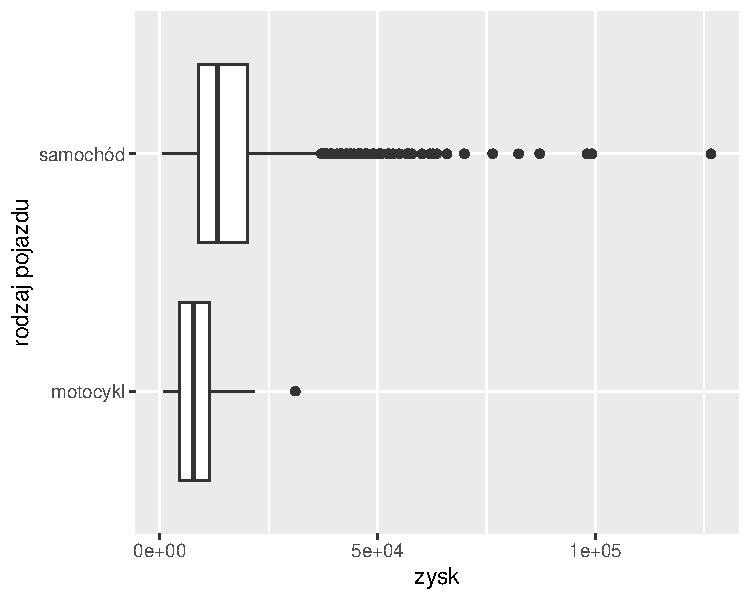
\includegraphics[width=\maxwidth]{figure/fig_typ-1} 

}

\caption[Wykresy pudełkowe zysku ze względu na rodzaj pojazdu]{Wykresy pudełkowe zysku ze względu na rodzaj pojazdu}\label{fig:fig_typ}
\end{figure}

\end{knitrout}

\subsection{Czy powypadkowy}

[tabelka z miarami ???]

\begin{knitrout}
\definecolor{shadecolor}{rgb}{0.969, 0.969, 0.969}\color{fgcolor}\begin{figure}

{\centering 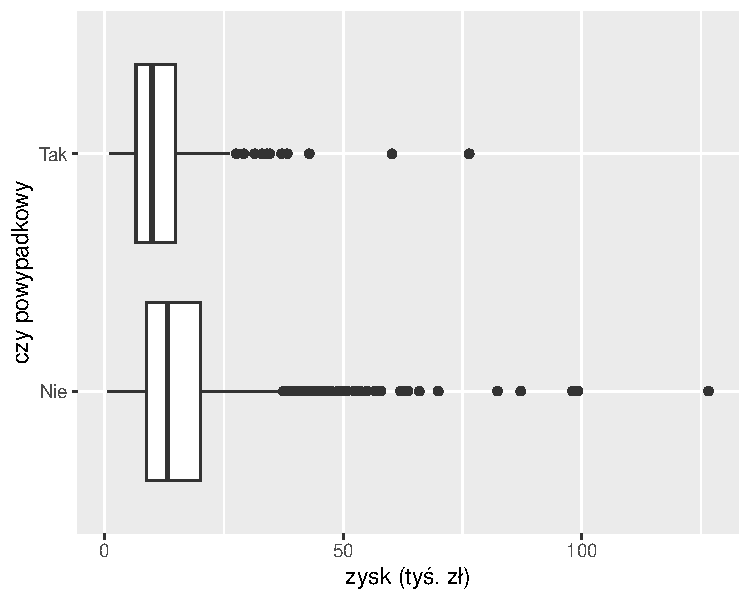
\includegraphics[width=\maxwidth]{figure/fig_wypadkowy-1} 

}

\caption[Wykresy pudełkowe zysku ze względu na to czy pojazd jest powypadkowy]{Wykresy pudełkowe zysku ze względu na to czy pojazd jest powypadkowy}\label{fig:fig_wypadkowy}
\end{figure}

\end{knitrout}

\subsection{skrzynia biegów / pojemność silnika}

[tabelka z miarami ???]

\begin{knitrout}
\definecolor{shadecolor}{rgb}{0.969, 0.969, 0.969}\color{fgcolor}

{\centering 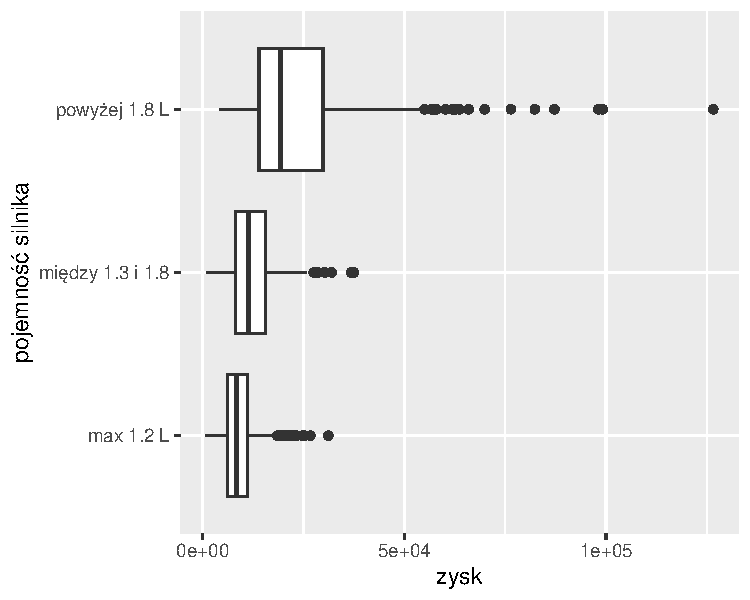
\includegraphics[width=\maxwidth]{figure/unnamed-chunk-8-1} 

}


\end{knitrout}




\end{document}
